% File: A.tex
% Created: 2014-11-07
% Author: Tesser Paolo
% Email: p.tesser921@gmail.com
% 
%
% Modification History
% Version	Modifier Date	Author			Change
% ====================================================================
% 0.0.1		2014-11-07		Tesser Paolo	inserita sezione
% ====================================================================
% 0.0.2		2015-02-03		Tesser Paolo	sistemata nota Amministratore, Ambiente di lavoro
% ====================================================================
% 0.0.3		2015-03-12		Tesser Paolo	inserito vocabolo: Anamnesi
% ====================================================================
%
\section{A}

\begin{itemize}
	\item \textbf{Ambiente di lavoro}: è ciò che serve ai processi di produzione. \'E composto da:
		\begin{itemize}
			\item persone
			\item ruoli
			\item procedure
			\item infrastrutture
		\end{itemize}
	\noindent
	Esso influisce sulla qualità del processo e del prodotto. Deve essere quindi: completo, ordinato e aggiornato;

	\item \textbf{Amministratore}: è uno dei ruoli di gestione di un progetto. Esso ha il compito di controllare l'ambiente di lavoro e di amministrare le infrastrutture necessarie allo svolgimento del progetto. \newline
	Deve mettere in pratica ciò che le norme chiedono e attraverso sistemi automatizzati le deve fare eseguire senza renderle troppo ingombranti per gli altri membri. Questo lavoro va fatto in maniera preventiva e pro attiva rispetto l'inizio delle attività e del tutto trasparente agli altri componenti. \newline
	A questa figura fanno quindi capo le configurazioni sui sistemi di versionamento e tutta la documentazione che viene redatta. Non attua scelte personali, ma segue quelle concordate con i responsabili;

	\item \textbf{Analisi vs. Progettazione}: [IS] generalmente l'approccio che abbiamo con l'analisi è di tipo top-down in quanto, se non si ha esperienza, non si riescono ad individuare da subito i componenti del sistema. \'E meglio quindi partire dalle richieste del proponente e ricavarne dei casi d'uso e dei requisiti che andranno a raffinarsi sempre di più. \newline
	Per quanto riguarda la progettazione invece si tende ad avere un approccio bottom-up dato che dopo l'analisi si hanno già in mente le componenti principale del sistema. \newline
	Nonostante quanto detto si possono individuare due tipi approccio:
		\begin{itemize}
			\item \textbf{Funzionale}: in questo caso, l'analisi usa prevalentemente il linguaggio naturale, mentre la specifica della progettazione usa linguaggi formali definendo le funzione e il profilo operazionale. Questo implica una progettazione top-down e una programmazione procedurale;
			\item \textbf{Object-oriented}: in questo caso, l'analisi è orientata agli oggetti, ne deriva un uso prevalente di formalismi grafici (Use Case). Questo implica una progettazione bottom-up, basata sul riuso di componenti già esistenti o la realizzazione di componenti riusabili. La programmazione sarà quindi OO.
		\end{itemize}

	\item \textbf{Analisi dinamica}: [VV] la ripetibilità in maniera deterministica è un requisito essenziale per questo tipo di analisi. Si devono utilizzare alcuni tipi di strumenti:
		\begin{itemize}
			\item \textbf{Driver}: componente attiva fittizia che serve a pilotare un parte del programma. (non è ciò che voglio testare)
			\item \textbf{Stub}: componente passiva fittizia per simulare una parte del programma. \'E un sostituto dell cose che devo guardare che restituisce però sempre la risposta giusta;
			\item \textbf{Logger}: componente non intrusivo di registrazione dei dati di esecuzione per analisi dei risultati.
		\end{itemize}
		\noindent
		Ci sono due tipi di approccio che utilizzano questi strumenti: \textbf{top-down} e \textbf{bottom-up}. Vediamo partendo dall'illustrazione seguente.
		\begin{figure}[htbp]
			\centering
			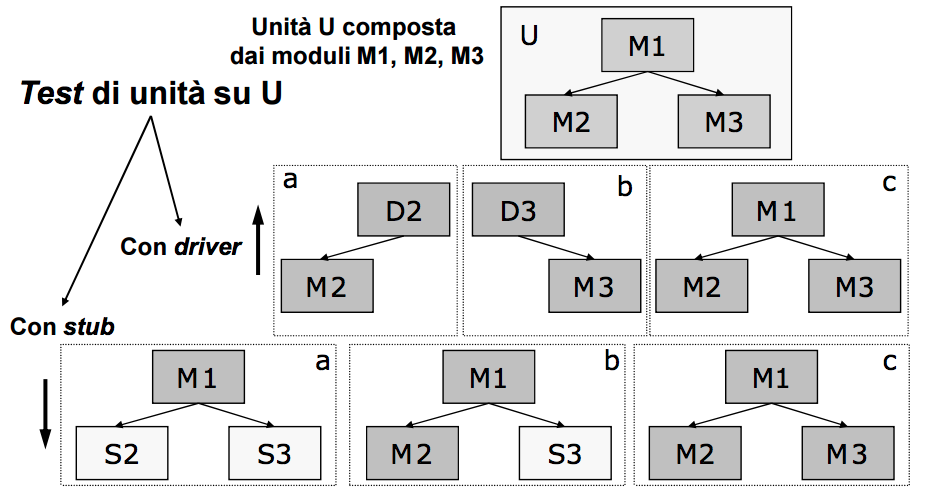
\includegraphics[scale=0.45]{img/stub_driver.png}
			\caption{Architettura Documentazione}
			\label{fig:arch_doc}
		\end{figure}
		Se lavoro in maniera \textbf{top-down} assumo che il comportamento delle foglie sia corretto grazie all'utilizzo di stub. Se invece lavoro in maniera \textbf{bottom-up} rimpiazzo la radice con un driver.







		\item \textbf{Analisi statica}: [VV] attività di verifica applicabile anche sui documenti. Non richiede l'esecuzione di parti del sistema SW. Viene applicata a ogni prodotto di processo e non solo al codice. Si può effettuare con metodi di lettura, impiegati solo per prodotti semplici, e metodi formali, basati sulla prova assistita di proprietà. Vediamo meglio nel dettaglio la parte che riguarda principalmente l'analisi statica del codice. \newline
		Un numero sempre maggiori di sistemi SW incorpora funzionalità critiche. \'E bene quindi essere in grado di sapere se un sistema è sicuro in maniera \textbf{safety}, cioè il sistema non fa danni, e in maniera \textbf{security}, cioè che sono protetto da intrusi. Il SW deve possedere tutte le capacità funzionali elencate nei requisiti e anche tutte le capacità non funzionali necessarie per garantire che il sistema lavori sempre come previsto, quindi non sul comportamento, ma sul modo in cui lo faccio. Per verificare quindi queste cose bisogna possedere, in maniera dimostrabile, determinata proprietà (di costruzione, d'uso, di funzionamento). \newline
		Nessun linguaggio di programmazione garantisce a priori la completa verificabilità di ogni programma scritto. Questo implica che scelto un linguaggio e valutati i suoi costrutti, bisogni porre dei vincoli di modi di programmazione nelle norme di progetto. Vediamo ora alcuni tipi di analisi statica:
			\begin{itemize}
				\item \textbf{Tracciamento}: serve a dimostrare la completezza ed economicità della soluzione. Questo implica il soddisfacimento di tutti i requisiti garantendo che non siano state create funzionalità superflue ed ingiustificate. Particolari stili di codifica facilitano la verifica mediante tracciamento. Assegnando singoli requisiti elementari a singoli moduli del programma;
				\item \textbf{Revisioni}: è uno strumento essenziale del processo di verifica. Possono essere condotte sull'analisi, la progettazione, il codice, procedure e risultati di verifica. Queste non sono automatizzabili. Possono essere formali o informali;
				\item \textbf{Flusso di controllo}: TODO;
				\item \textbf{Flusso di dati}: TODO;
				\item \textbf{Flusso dell'informazione}: TODO;
				\item \textbf{Esecuzione simbolica}: TODO;
				\item \textbf{Verifica formale del codice}: TODO;
				\item \textbf{Verifica di limite}: TODO;
				\item \textbf{Uso dello stack}: TODO;
				\item \textbf{Comportamento temporale}: TODO;
				\item \textbf{Interferenza}: TODO;
				\item \textbf{Codice oggetto}: TODO.
			\end{itemize}




	\item \textbf{Analista}: è uno dei ruoli di gestione di un progetto. Esso ha il compito di capire il problema per ottenere i requisiti. Non da la soluzione e spesso non segue fino in fondo la realizzazione del progetto, ma è presente principalmente nella fase iniziale. \newline
	Per cercare i requisiti segue un approccio top-down. Parte infatti ad analizzare quelli espliciti del proponente fino a scinderli in vari sottogruppi gerarchici, trovandone nel frattempo anche di impliciti (il numero maggiore tra le due tipologie);

	\item \textbf{Anamnesi}: nella filosofia platonica è quel processo di reminiscenza che, stimolato dalla percezione degli oggetti sensibili, conduce l'uomo a riscoprire gradualmente nel proprio intelletto (attraverso la conoscenza intellettiva) quelle idee eterne che sono causa e origine del mondo fenomenico. La conoscenza sensibile, distinta dalla conoscenza intellettiva, può dunque offrire a quest'ultima lo spunto per avviare un tale processo;

	\item \textbf{Architettura}: [PR] (definizione) Prima degli anni 80 il termine architettura veniva applicato prevalentemente al sistema fisico. Viene riconosciuto anche nell'ambito software dopo l'evento che riconosceva la disciplina stessa del software engineering. \newline
	Viene definita quindi come una collezione di software e componenti del sistema che dialogano tramite connessioni soggette a vincoli. Questo, quando implementate, andranno a soddisfare le necessità degli stakeholders. Un sistema di architettura software comprende:
		\begin{itemize}
			\item l'insieme di decisioni sull'organizzazione del sistema software;
			\item la selezione degli elementi strutturali e la loro interfaccia con il sistema;
			\item la composizione di queste strutture e il comportamento degli elementi in un sempre più ampio sotto insieme;
			\item lo stile architetturale che guida l'organizzazione. Faccio così perché ottengo questo.
		\end{itemize}
		\noindent
	La decomposizione del sistema in componenti deve essere fatta in maniera top-down. I componenti devono anche essere organizzati in modo da definirne ruoli, responsabilità e interazioni. Buone scelte quindi permettono una buona manutenibilità;

	\item \textbf{Architettura della documentazione}: [DOC] TODO
		\begin{figure}[htbp]
			\centering
			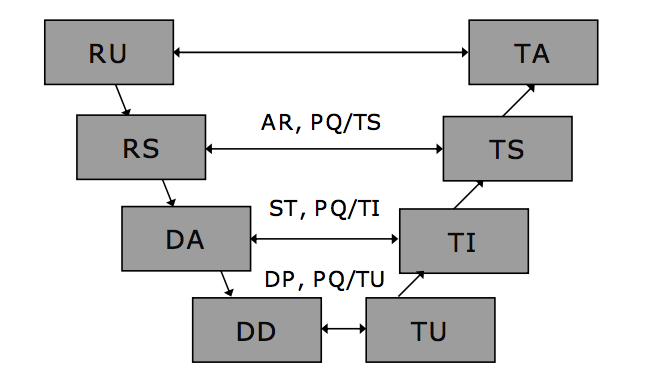
\includegraphics[scale=0.6]{img/v_model_tullio.png}
			\caption{V Model}
			\label{fig:v_model}
		\end{figure}

\end{itemize}
